% Title: gl2ps_renderer figure
% Creator: GL2PS 1.4.0, (C) 1999-2017 C. Geuzaine
% For: Octave
% CreationDate: Mon Apr 26 23:22:55 2021
\setlength{\unitlength}{1pt}
\begin{picture}(0,0)
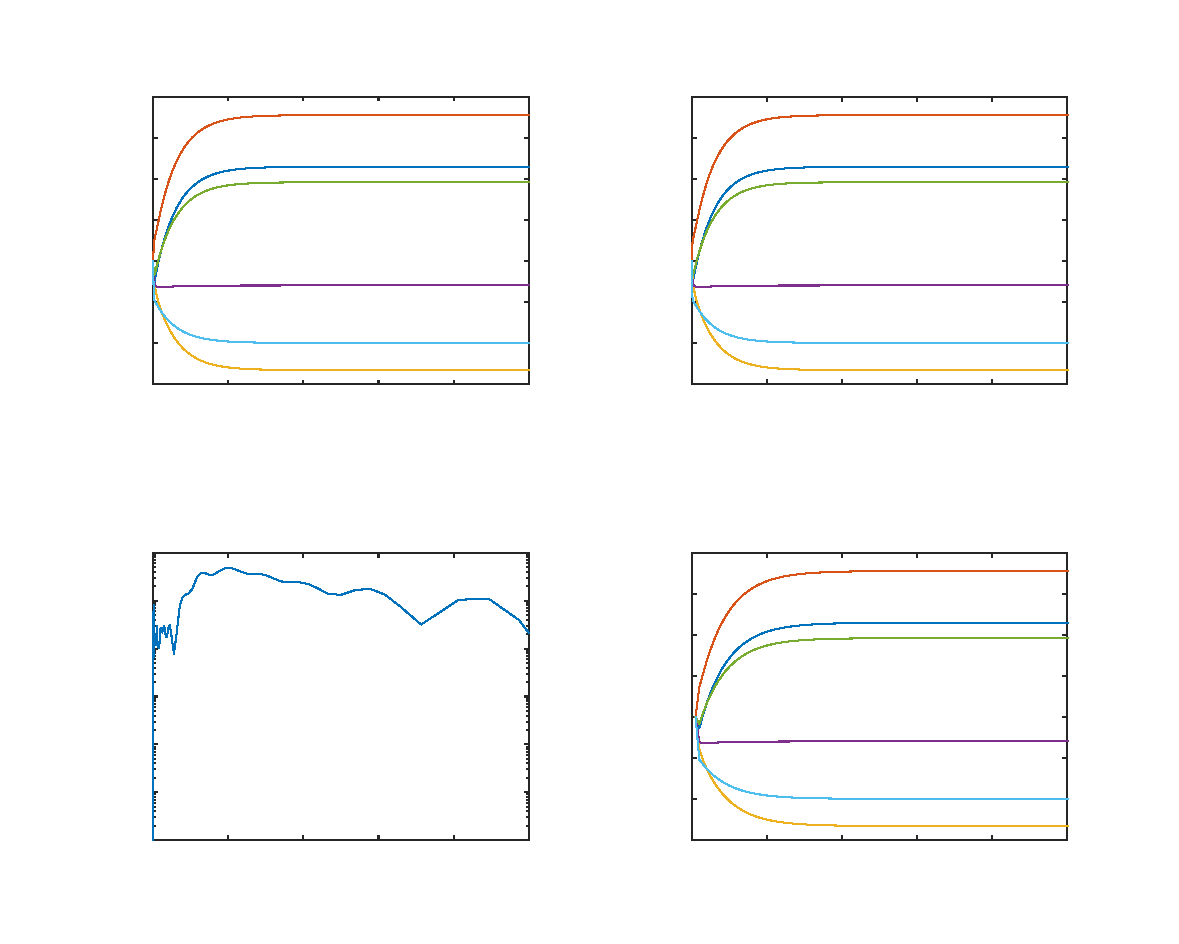
\includegraphics{Trajectory-inc}
\end{picture}%
\begin{picture}(566,453)(0,0)
\fontsize{10}{0}
\selectfont\put(73.5801,254.606){\makebox(0,0)[t]{\textcolor[rgb]{0.15,0.15,0.15}{{0}}}}
\fontsize{10}{0}
\selectfont\put(111.151,254.606){\makebox(0,0)[t]{\textcolor[rgb]{0.15,0.15,0.15}{{20}}}}
\fontsize{10}{0}
\selectfont\put(148.722,254.606){\makebox(0,0)[t]{\textcolor[rgb]{0.15,0.15,0.15}{{40}}}}
\fontsize{10}{0}
\selectfont\put(186.293,254.606){\makebox(0,0)[t]{\textcolor[rgb]{0.15,0.15,0.15}{{60}}}}
\fontsize{10}{0}
\selectfont\put(223.865,254.606){\makebox(0,0)[t]{\textcolor[rgb]{0.15,0.15,0.15}{{80}}}}
\fontsize{10}{0}
\selectfont\put(261.436,254.606){\makebox(0,0)[t]{\textcolor[rgb]{0.15,0.15,0.15}{{100}}}}
\fontsize{10}{0}
\selectfont\put(68.584,262.103){\makebox(0,0)[r]{\textcolor[rgb]{0.15,0.15,0.15}{{-2}}}}
\fontsize{10}{0}
\selectfont\put(68.584,281.81){\makebox(0,0)[r]{\textcolor[rgb]{0.15,0.15,0.15}{{-1}}}}
\fontsize{10}{0}
\selectfont\put(68.584,301.517){\makebox(0,0)[r]{\textcolor[rgb]{0.15,0.15,0.15}{{0}}}}
\fontsize{10}{0}
\selectfont\put(68.584,321.224){\makebox(0,0)[r]{\textcolor[rgb]{0.15,0.15,0.15}{{1}}}}
\fontsize{10}{0}
\selectfont\put(68.584,340.93){\makebox(0,0)[r]{\textcolor[rgb]{0.15,0.15,0.15}{{2}}}}
\fontsize{10}{0}
\selectfont\put(68.584,360.637){\makebox(0,0)[r]{\textcolor[rgb]{0.15,0.15,0.15}{{3}}}}
\fontsize{10}{0}
\selectfont\put(68.584,380.344){\makebox(0,0)[r]{\textcolor[rgb]{0.15,0.15,0.15}{{4}}}}
\fontsize{10}{0}
\selectfont\put(68.584,400.051){\makebox(0,0)[r]{\textcolor[rgb]{0.15,0.15,0.15}{{5}}}}
\fontsize{11}{0}
\selectfont\put(167.508,410.051){\makebox(0,0)[b]{\textcolor[rgb]{0,0,0}{{gsl solution in C}}}}
\fontsize{11}{0}
\selectfont\put(54.584,331.077){\rotatebox{90}{\makebox(0,0)[b]{\textcolor[rgb]{0.15,0.15,0.15}{{x(t)}}}}}
\fontsize{11}{0}
\selectfont\put(167.508,241.606){\makebox(0,0)[t]{\textcolor[rgb]{0.15,0.15,0.15}{{t}}}}
\fontsize{10}{0}
\selectfont\put(324.374,254.606){\makebox(0,0)[t]{\textcolor[rgb]{0.15,0.15,0.15}{{0}}}}
\fontsize{10}{0}
\selectfont\put(361.945,254.606){\makebox(0,0)[t]{\textcolor[rgb]{0.15,0.15,0.15}{{20}}}}
\fontsize{10}{0}
\selectfont\put(399.517,254.606){\makebox(0,0)[t]{\textcolor[rgb]{0.15,0.15,0.15}{{40}}}}
\fontsize{10}{0}
\selectfont\put(437.088,254.606){\makebox(0,0)[t]{\textcolor[rgb]{0.15,0.15,0.15}{{60}}}}
\fontsize{10}{0}
\selectfont\put(474.659,254.606){\makebox(0,0)[t]{\textcolor[rgb]{0.15,0.15,0.15}{{80}}}}
\fontsize{10}{0}
\selectfont\put(512.23,254.606){\makebox(0,0)[t]{\textcolor[rgb]{0.15,0.15,0.15}{{100}}}}
\fontsize{10}{0}
\selectfont\put(319.378,262.103){\makebox(0,0)[r]{\textcolor[rgb]{0.15,0.15,0.15}{{-2}}}}
\fontsize{10}{0}
\selectfont\put(319.378,281.81){\makebox(0,0)[r]{\textcolor[rgb]{0.15,0.15,0.15}{{-1}}}}
\fontsize{10}{0}
\selectfont\put(319.378,301.517){\makebox(0,0)[r]{\textcolor[rgb]{0.15,0.15,0.15}{{0}}}}
\fontsize{10}{0}
\selectfont\put(319.378,321.224){\makebox(0,0)[r]{\textcolor[rgb]{0.15,0.15,0.15}{{1}}}}
\fontsize{10}{0}
\selectfont\put(319.378,340.93){\makebox(0,0)[r]{\textcolor[rgb]{0.15,0.15,0.15}{{2}}}}
\fontsize{10}{0}
\selectfont\put(319.378,360.637){\makebox(0,0)[r]{\textcolor[rgb]{0.15,0.15,0.15}{{3}}}}
\fontsize{10}{0}
\selectfont\put(319.378,380.344){\makebox(0,0)[r]{\textcolor[rgb]{0.15,0.15,0.15}{{4}}}}
\fontsize{10}{0}
\selectfont\put(319.378,400.051){\makebox(0,0)[r]{\textcolor[rgb]{0.15,0.15,0.15}{{5}}}}
\fontsize{11}{0}
\selectfont\put(418.302,410.051){\makebox(0,0)[b]{\textcolor[rgb]{0,0,0}{{analytical solution}}}}
\fontsize{11}{0}
\selectfont\put(305.378,331.077){\rotatebox{90}{\makebox(0,0)[b]{\textcolor[rgb]{0.15,0.15,0.15}{{$x(t)$}}}}}
\fontsize{11}{0}
\selectfont\put(418.302,241.606){\makebox(0,0)[t]{\textcolor[rgb]{0.15,0.15,0.15}{{$t$}}}}
\fontsize{10}{0}
\selectfont\put(73.5801,42.333){\makebox(0,0)[t]{\textcolor[rgb]{0.15,0.15,0.15}{{0}}}}
\fontsize{10}{0}
\selectfont\put(111.151,42.333){\makebox(0,0)[t]{\textcolor[rgb]{0.15,0.15,0.15}{{20}}}}
\fontsize{10}{0}
\selectfont\put(148.722,42.333){\makebox(0,0)[t]{\textcolor[rgb]{0.15,0.15,0.15}{{40}}}}
\fontsize{10}{0}
\selectfont\put(186.293,42.333){\makebox(0,0)[t]{\textcolor[rgb]{0.15,0.15,0.15}{{60}}}}
\fontsize{10}{0}
\selectfont\put(223.865,42.333){\makebox(0,0)[t]{\textcolor[rgb]{0.15,0.15,0.15}{{80}}}}
\fontsize{10}{0}
\selectfont\put(261.436,42.333){\makebox(0,0)[t]{\textcolor[rgb]{0.15,0.15,0.15}{{100}}}}
\fontsize{10}{0}
\selectfont\put(68.584,49.8301){\makebox(0,0)[r]{\textcolor[rgb]{0.15,0.15,0.15}{{$10^{-9}$}}}}
\fontsize{10}{0}
\selectfont\put(68.584,95.8125){\makebox(0,0)[r]{\textcolor[rgb]{0.15,0.15,0.15}{{$10^{-8}$}}}}
\fontsize{10}{0}
\selectfont\put(68.584,141.795){\makebox(0,0)[r]{\textcolor[rgb]{0.15,0.15,0.15}{{$10^{-7}$}}}}
\fontsize{10}{0}
\selectfont\put(68.584,187.777){\makebox(0,0)[r]{\textcolor[rgb]{0.15,0.15,0.15}{{$10^{-6}$}}}}
\fontsize{11}{0}
\selectfont\put(167.508,197.777){\makebox(0,0)[b]{\textcolor[rgb]{0,0,0}{{Difference between gsl and analytical solution}}}}
\fontsize{11}{0}
\selectfont\put(22.584,118.804){\rotatebox{90}{\makebox(0,0)[b]{\textcolor[rgb]{0.15,0.15,0.15}{{$\sum_i |x_i(t) - x_i(t;\texttt{gsl})|$}}}}}
\fontsize{11}{0}
\selectfont\put(167.508,29.333){\makebox(0,0)[t]{\textcolor[rgb]{0.15,0.15,0.15}{{$t$}}}}
\fontsize{10}{0}
\selectfont\put(324.374,42.333){\makebox(0,0)[t]{\textcolor[rgb]{0.15,0.15,0.15}{{0}}}}
\fontsize{10}{0}
\selectfont\put(361.945,42.333){\makebox(0,0)[t]{\textcolor[rgb]{0.15,0.15,0.15}{{20}}}}
\fontsize{10}{0}
\selectfont\put(399.517,42.333){\makebox(0,0)[t]{\textcolor[rgb]{0.15,0.15,0.15}{{40}}}}
\fontsize{10}{0}
\selectfont\put(437.088,42.333){\makebox(0,0)[t]{\textcolor[rgb]{0.15,0.15,0.15}{{60}}}}
\fontsize{10}{0}
\selectfont\put(474.659,42.333){\makebox(0,0)[t]{\textcolor[rgb]{0.15,0.15,0.15}{{80}}}}
\fontsize{10}{0}
\selectfont\put(512.23,42.333){\makebox(0,0)[t]{\textcolor[rgb]{0.15,0.15,0.15}{{100}}}}
\fontsize{10}{0}
\selectfont\put(319.378,49.8301){\makebox(0,0)[r]{\textcolor[rgb]{0.15,0.15,0.15}{{-2}}}}
\fontsize{10}{0}
\selectfont\put(319.378,69.5366){\makebox(0,0)[r]{\textcolor[rgb]{0.15,0.15,0.15}{{-1}}}}
\fontsize{10}{0}
\selectfont\put(319.378,89.2437){\makebox(0,0)[r]{\textcolor[rgb]{0.15,0.15,0.15}{{0}}}}
\fontsize{10}{0}
\selectfont\put(319.378,108.95){\makebox(0,0)[r]{\textcolor[rgb]{0.15,0.15,0.15}{{1}}}}
\fontsize{10}{0}
\selectfont\put(319.378,128.657){\makebox(0,0)[r]{\textcolor[rgb]{0.15,0.15,0.15}{{2}}}}
\fontsize{10}{0}
\selectfont\put(319.378,148.364){\makebox(0,0)[r]{\textcolor[rgb]{0.15,0.15,0.15}{{3}}}}
\fontsize{10}{0}
\selectfont\put(319.378,168.071){\makebox(0,0)[r]{\textcolor[rgb]{0.15,0.15,0.15}{{4}}}}
\fontsize{10}{0}
\selectfont\put(319.378,187.777){\makebox(0,0)[r]{\textcolor[rgb]{0.15,0.15,0.15}{{5}}}}
\fontsize{11}{0}
\selectfont\put(418.302,197.777){\makebox(0,0)[b]{\textcolor[rgb]{0,0,0}{{lsode solution in \emph{GNU Octave}}}}}
\fontsize{11}{0}
\selectfont\put(305.378,118.804){\rotatebox{90}{\makebox(0,0)[b]{\textcolor[rgb]{0.15,0.15,0.15}{{$x(t)$}}}}}
\fontsize{11}{0}
\selectfont\put(418.302,29.333){\makebox(0,0)[t]{\textcolor[rgb]{0.15,0.15,0.15}{{$t$}}}}
\end{picture}
